%    Copyright and Patent Pending (C) 2012, Troy Benjegerdes
%
%    This program, which is a patent and software to specify a physical
%    hardware platform is free software: you can redistribute it and/or modify
%    it, or any derived work under the terms of the GNU Affero General Public
%    License as published by the Free Software Foundation, either version 3 of
%    the License, or (at your option) any later version.
%
%    This program is distributed in the hope that it will be useful,
%    but WITHOUT ANY WARRANTY; without even the implied warranty of
%    MERCHANTABILITY or FITNESS FOR A PARTICULAR PURPOSE.  See the
%    GNU Affero General Public License for more details.
%
%    You should have received a copy of the GNU Affero General Public License
%    along with this program.  If not, see <http://www.gnu.org/licenses/>.


% this patent application is derived from a public domain template, of 
% which the original header is below:
%%%%%%%%%%%%%%%%%%%%%%%%%%%%%%%%%%%%%%%%%%%%%%%%%%%%%%%%%%%%%%%%%%%%%%%%%%%%%%
%                                                            12.18.18.12.19
%                                                          13 CAUAC  7 KANKIN
%                                                          ( January 1, 1992 )
%
%   This file is a template for preparing patent applications.  It includes
% sections for all of the important aspects of a patent application, including
% the patent specification, claims, abstract, figures, and other parts. The
% file uses the LaTeX layout program. The margin settings and line spacing are
% set to conform to requirements of the US Patent Office, when the text is
% printed out on 8.5 by 11 inch paper.
%
%   This file makes use of other files which are included in the processing
% by use of the TeX command \input{}.  These files are:
%		objects.tex
%		figures.tex
%		broadly.tex
%		claims.tex
%
%   This is version 0.5 of these files.  Please send any comments and
% suggestions to Gregory Aharonian,  srctran@world.std.com, to be included
% in future releases of this template.  My goal is to be able to offer to
% people enough of a temple, which when used with a very excellent book,
% "Patent It Yourself" by David Pressman (Nolo Press, Berkeley, CA), should
% help people prepare their own patents. Also a good template might coax the
% Patent Office into accepting machine readable patent specifications.
%
%%%%%%%%%%%%%%%%%%%%%%%%%%%%%%%%%%%%%%%%%%%%%%%%%%%%%%%%%%%%%%%%%%%%%%%%%%%%%%

%\documentclass[times,twocolumn]{article}
\documentclass[times]{article}
\usepackage{times}
\usepackage{graphicx}

\begin{document}

\begin{center}
{\bf ABSTRACT: ~~~~~~~AMMONIA COOLED HIGH PERFORMANCE COMPUTER}
\end{center}

A method for system optimization and performance improvement of high performance
computing systmes is disclosed in which individual, modular compute elements are
fully encased in a hermetically sealed heat-conductive casing, aggregated around
cooling tubes, and powered by a single cable which provides both power and high
performance computing interconnect capability. Further, the system is operated
to dynamically balance computing performance with thermodynamic system parameters,
depending on various conditions, including renewable energy availability and
real-time energy market conditions.

\begin{figure}
\begin{center}
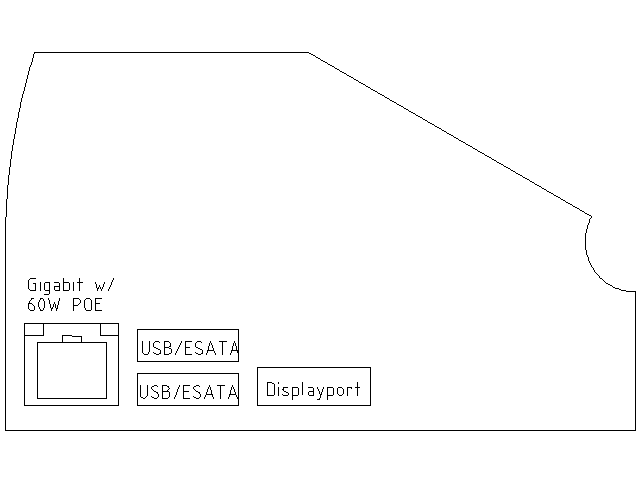
\includegraphics[width=\columnwidth]{cube}
\caption{The Q3ube Building Block}
\label{cube}
\end{center}
\end{figure}

\begin{figure}
\begin{center}
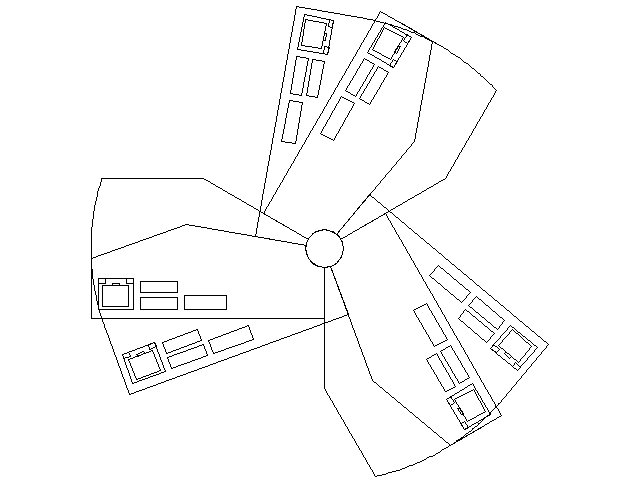
\includegraphics[width=\columnwidth]{supercube}
\caption{Compute cluster around heat removal piping}
\label{supercube}
\end{center}
\end{figure}

\begin{center}
Patent Application

of

Troy Benjegerdes

for

{\bf The Q3ube: AMMONIA COOLED COMPUTING EQUIPMENT}

of which the following is a specification:

---

\end{center}

{\bf FREE SOFTWARE COPYRIGHT NOTICE}
This patent is a derivative work of a free software program: you can redistribute
it and/or modify it under the terms of the GNU Affero General Public License as
published by the Free Software Foundation, either version 3 of the License, or
(at your option) any later version.

Distribution of the derived works of the program (this patent application in 
html, pdf, or other format) without making available the full program specification,
or minimally, without the source human-modifiable .tex files is subject to a license
fee of \$250,000 USD per incident. Recipients of this PDF file are advised that they
may be liable for copying performed on their behalf by cloud computing service providers.

Only the author (currently only Troy Benjegerdes) or his direct contractors or 
assignees may distribute the derived works file without corresponding .tex source
code. The Internet Archive (archive.org) is specifically granted a license to archive
this derived work in html form. All other rights are strictly reserved and subject
to advertised copyright license fees as above.

% SKIPSKIP
\begin{center}
{\bf FIELD OF THE INVENTION}
\end{center}
% SKIPSKIP

   The present invention pertains generally to use of Ammonia (NH3) for cooling,
and more particularly to a method of cooling computing equipment.

\begin{center}
{\bf BACKGROUND OF THE INVENTION}
\end{center}

   Ammonia is a widely used synthetic compound, with primary use as fertilizer,
along with many important uses in chemical synthesis, refrigeration. It has been
heavily used in industrial refrigeration due to the very high heat of vaporization,
which is surpassed only by that of water. All other commonly used refrigerants and
cooling fluids have a significantly lower heat capacity. This invention uses a 
commodity standard building block which can be utilized as a fanless desktop computer
replacment, or aggregated around a heat removal pipe which may carry water, ammonia,
or some other fluid. For even higher performance, the basic commidity building block
can be sealed with an appropriate sealant and fully submerged in pressurized liquid
ammonia. Temperature of the computing elements can be easily controlled by a pressure
control valve, which changes the effective boiling point of the cooling liquid.


\begin{center}
{\bf SUMMARY OF THE INVENTION}
\end{center}

% This section briefly discusses the new invention, and starts out with a
% formal statement of what the new invention does in terms of "objects".

\input{objects}

% Once the objects of the invention are stated, then you can include a
% review of what the new invention does.  Often this review is written
% informally, since a detailed description is required further on.


\begin{center}
{\bf DESCRIPTION OF PRIOR ART}
\end{center}

 * reference cray patents on cooling *

Additionally, the inventor, Troy Benjegerdes has published prior art
for the concept of software systems which adapt to real-time power market
or renewable energy availability. This prior art was primarily published
via the http://Grid.coop domain name, registered April, 2008, and the
Iowa Power Fund application entitled 'Iowa Grid: Open source infrastructure
for time-of-day and location-based electric power trading', submitted
to the Iowa Power fund on or about March 18, 2008.

{\bf(can we incorporate the power fund application by reference??)}


% ****************************************************************************
% The vast majority of patents include figures illustrating the design of the
% new invention. These figures have to be prepared according to Patent Office
% rules.  While you can initially submit informal drawings (hand drawn, output
% from a CAD program), eventually you have to sumit formal drawings.  However
% in most cities you can hire patent draftspeople who will prepare formal
% drawings for about one hundred dollars per page.

\input{figures}

%
% ****************************************************************************


% Detail description, in the form of a narrative
\input{detail}


% ****************************************************************************
% You should have a paragraph declaring that not only are you claiming what is
% described in this patent specification, but also anything that is an obvious
% variation, modification or extension of the invention.  For example, stating
% that the bicycle wheel uses say, three spokes, shouldn't limit you to
% wheel with three spokes. This 'broadening' sections helps you avoid claiming
% three spokes, four spokes, five spokes, etc.
%

\input{broadly}

%
% ****************************************************************************


%
%  The Patent Office operates a service to register the fact that you have
% invented something, that you will be patenting the invention, but want to
% have an official record of the date you discovered the invention. To do
% so, prepare a detailed description of your invention, and submit it to the
% Patent Office (along with a check for six dollars).  A few weeks later you
% will receive a letter informing you that the Patent Office has you notice
% of discovery on file, along with a identifying number, to be used when you
% file the patent application.  The files DISCLOSE.DOC and DISCLOSE.PAT have
% additional instructions on using this service.
%

\begin{center}
{CROSS REFERENCE TO DISCLOSURE DOCUMENT}
\end{center}


\newpage

% ****************************************************************************
% Most of the patent application, while required and useful for defending your
% patent intentions in court, pale in comparison to the importance of the
% claims section of your patent. Writing patent claims is not trivial. There
% are certain words that should be used, and ways that previous claims refer
% back to earlier claims. Be careful, read anything you can on writing claims,
% and consult a lawyer is this process is confusing.
%

\input{claims}

%
% ****************************************************************************

\newpage

\end{document}
